\section*{\hypertarget{gm}{Director del Juego}}
"Sin embargo, no nos culpes a nosotros.\newline Cúlpate a ti mismo o a Dios".\\
\indent -- Delita

\begin{center} 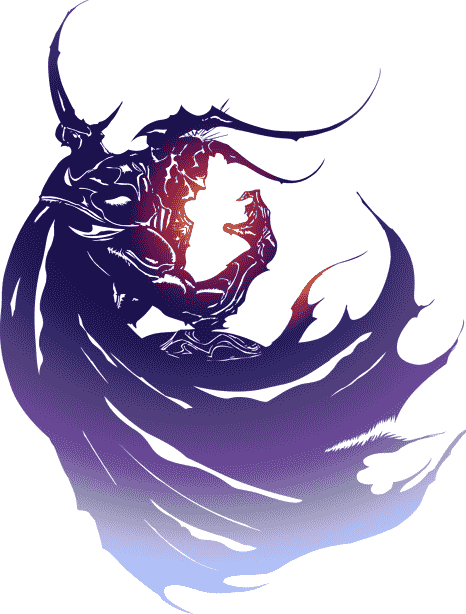
\includegraphics[width=\columnwidth]{./art/images/ff4.png} \end{center}
%
\addcontentsline{toc}{section}{Director del Juego}
%
El Director del Juego (DJ) tiene un papel diferente al de los jugadores. Estos últimos juegan desde la perspectiva de los protagonistas. El DJ, en cambio, crea el mundo y el entorno de la aventura y asume el papel de todos los personajes que no son jugadores. Además, el DJ describe el ambiente y narra los resultados de todas las acciones. Esta sección tiene una serie de guías que ayudarán a los DJ a comprender mejor su función. Además, incluye una gran variedad de contenidos que puedes utilizar para crear el mundo de tu juego.

\subsubsection*{Sesiones}
La mayoría de las aventuras son demasiado largas como para completarlas en una sola sentada, por lo que deben dividirse en varias sesiones. Por lo tanto, basta con preparar el contenido solo para la próxima sesión, en lugar de todo con antelación. Durante el juego, busca oportunidades para finalizar una sesión en curso con algún hecho importante (por ejemplo, después de concluir una misión). Se pueden planificar las sesiones de acuerdo con los \hyperlink{ms}{Hitos} de la aventura, que marcan la subida de nivel de los personajes (deberían subir de nivel una vez de cada 1 a 3 sesiones). Aun así, no podrás estar preparado para todo, así que no tengas miedo de improvisar cuando sea necesario.

\pagebreak

\subsubsection*{Tiradas}
Las tiradas son una herramienta poderosa que te ayuda a decidir el resultado de acciones inciertas. Cuando los jugadores intenten realizar alguna acción, puedes pedirles que hagan una tirada y asignar una DC secreta a la tarea. En algunas situaciones, también puedes pedir directamente a los jugadores que hagan tiradas, p. ej., para decidir si el grupo se da cuenta o no que se dirigen hacia una emboscada. Todos los personajes no jugadores controlados por ti también tienen que hacer sus tiradas ya que se rigen por las mismas reglas. Sin embargo, no tienes que hacer tiradas si el resultado de una acción es demasiado evidente.

\subsubsection*{Combate}
Durante el combate, interpretas el papel de todos los personajes no jugadores y todas las \hyperlink{combat}{Reglas de combate} se aplican a ellos también. A diferencia de los jugadores, puedes mantener la mayor parte de la información en secreto, como los PV y PM restantes y las tiradas de dados. Cuando interpretes a un grupo enemigo, debes tomar decisiones desde su perspectiva, sin utilizar tus propios conocimientos. Al crear batallas, intenta equilibrar el número de participantes de ambos bandos. Las grandes hordas de enemigos débiles a menudo desbordarán al grupo, mientras que un solo enemigo fuerte puede no tener oportunidad alguna. Una mezcla saludable de distintos enemigos hace que el combate sea más interesante. Además, puedes utilizar ayudas visuales (por ejemplo, un mapa) para hacer un seguimiento del campo de batalla. Las batallas son una cuestión de vida o muerte, por lo que normalmente llevan bastante tiempo en una sesión. Por lo tanto, intenta centrarte en las batallas importantes de la aventura.

\subsubsection*{Narración y Roleo}
Para que tú y los jugadores logren sumergirse en el mundo que creaste, trata de dar descripciones breves y vívidas del entorno que rodea al grupo. Al hacerlo, haz hincapié en los elementos con los que los jugadores puedan interactuar de forma interesante. Así mismo, utiliza las descripciones que los jugadores hacen sobre las acciones de su personaje para crear tus narraciones sobre el resultado. Esto a menudo requiere que asumas el rol de muchos personajes diferentes para que interactúen con el grupo. En ese caso, trata de entender la perspectiva del personaje para reflejar cómo hablaría y actuaría cuando interactúa con el grupo.

\vspace{1cm} 

\example{Uso de las Tiradas}{
Zidane y Blank intentan representar convincentemente una lucha con espadas para un público de nobles. El DJ decide que esta es una tarea difícil (DC 9), porque las expectativas de los nobles son elevadas. Zidane tira 2d con el resultado 9, por lo que apenas pasa la tirada. En consecuencia, el DJ decide que la mayoría de los nobles están contentos con la actuación. Sin embargo, la reina Brahne no está impresionada. 
}

\pagebreak

\subsubsection*{Viajes y Tiempo}
Los jugadores pueden familiarizarse con el mundo explorando distintos lugares. Sin embargo, viajar a pie no siempre es la mejor opción debido al terreno difícil, al tiempo o a las emboscadas. Según el entorno de la aventura, pueden disponer de medios de transporte más cómodos, como barcos, trenes, aeronaves, automóviles o \hyperlink{chocobo}{Chocobos}. Por lo general, el grupo debe contratar dichos servicios, pero a medida que se hacen más ricos, pueden adquirir sus propios vehículos. Para viajes más largos, trata de hacer un seguimiento del tiempo que pasa y de cómo afecta al resto del mundo. En general, el tiempo pasa a una velocidad diferente en el juego que en la mesa. Esto se debe a que los aspectos intrascendentes de la aventura pueden ser narrados rápidamente, mientras que las decisiones importantes deben considerarse con más cuidado.

\subsubsection*{Riqueza}
Puedes dar a los jugadores Gil, objetos y equipo como incentivo para que completen determinadas tareas. En general, estas recompensas deben dividirse de forma equitativa entre todos los miembros del grupo. Otra forma de que los jugadores pueden generar riquezas es comerciar con personajes no jugadores. Por lo general, los comerciantes intentan vender los artículos por encima de su valor original y comprarlos a no más de la mitad de su valor original para que les sea rentable. Además, puedes modificar el costo que tiene descansar en una posada o una carpa para ajustar la dificultad del juego.

\vspace{1cm}

\example{Narración y Roleo}
{
\begin{description}[leftmargin=*]
 \item[Yasumi (DJ):] Al entrar en el Castillo Riovanes, se encuentran dentro de un gran salón con estrechas corrientes de agua en ambos costados. Entre los múltiples caballeros muertos que yacen dispersos en el suelo, observan que hay un hombre de pie al final de la escalera central. Se da vuelta y ven que es nada menos que... ¡Wiegraf Folles!
 \item[Yasumi (interpretando a Wiegraf):] Aquí estás,  \\ Ramza. Desenfunda tu espada.
 \item[Akihiko:] No desenfundo mi espada por ahora. Quizás podamos resolver esto pacíficamente.
 \item[Yasumi (interpretando a Wiegraf):] ¿Qué sucede? Si no lo haces, yo lo haré.
 \item[Akihiko (interpretando a Ramza):] Eres un miserable. Estás entregando tu espíritu a cambio de tu venganza.
 \item[Yasumi (interpretando a Wiegraf):] ¿Venganza? No busco venganza. Quiero sembrar el caos en todo el mundo. Pero no te preocupes. ¡Yo mismo voy a matarte!
 \item[Akihiko:] Bien, ¡ahora sí desenfundo mi espada!
 \item[Yasumi:] De acuerdo, vamos a hacer la tirada de iniciativa.
	\end{description}
}

\pagebreak

\subsubsection*{Misiones secundarias}
Si bien la aventura debería enfocarse en resolver el conflicto central, una sesión que vaya por fuera de la misión principal puede ser útil para aliviar la tensión. La lista de abajo muestra algunas ideas de tramas para misiones secundarias cortas.
\begin{description}[leftmargin=*]
 \item[\color{accent} Casino:] El grupo encuentra un extravagante casino que ofrece varios juegos de azar. Aunque no lo aparente al principio, jamás encontrarás un lugar más lleno de escorias y villanos. Si el grupo quiere jugar, puede realizar tiradas muy difíciles para decidir el resultado. Sin embargo, todos los juegos están arreglados en contra de los jugadores, por lo que es casi imposible obtener beneficios.
 \item[\color{accent} Granja de Chocobos:] El grupo encuentra una granja de \hyperlink{chocobo}{Chocobos}. El granjero es agradable y se disculpa por no poder alquilar sus Chocobos por el momento. Menciona que últimamente algunos de ellos han estado desapareciendo por la noche y está desesperado por resolver el misterio. Si el grupo encuentra la causa de su desaparición, el granjero muestra su gratitud prestando sus Chocobos de forma gratuita.
 \item[\color{accent} Coliseo:] El grupo llega a las puertas del Coliseo, un estadio donde los aventureros luchan contra monstruos y otros aventureros a modo de espectáculo. El propietario del establecimiento ofrece recompensas generosas al grupo por participar. Si acepta, el grupo tiene que luchar en múltiples batallas consecutivas, donde el fracaso significa una muerte certera. Además, la mayoría de los espectadores realizan apuestas sobre las batallas. El grupo puede intentar utilizar esto para su beneficio.
 \item[\color{accent} Maestro Artesano:] El grupo encuentra un taller atendido por un hombre llamado Cid. Cid es un maestro artesano (puede ser, por ejemplo, un mecánico o un herrero). Se queja con el grupo de que no puede trabajar porque no están llegando las entregas de materiales. Les ofrece sus servicios como recompensa si consiguen traerle algunos materiales raros.
 \item[\color{accent} Cueva Misteriosa:] El grupo se encuentra con dos soldados llamados Biggs y Wedge. A los dos se les asignó la tarea de encontrar un grupo de investigadores que han desaparecido en una cueva cercana. Se ven muy asustados, por lo que ofrecen la mitad de la recompensa por su ayuda. Parecen saber más sobre este incidente de lo que están diciendo.
 \item[\color{accent} Devorador de Zonas:] Una versión mucho más grande del \hyperlink{abyssworm}{Gusano de Arena} llamado "Devorador de Zonas" sorprende al grupo. A pesar de cualquier esfuerzo, la bestia se traga al grupo y los aventureros se encuentran dentro de su aparentemente infinito estómago. Se dan cuenta rápidamente de que no son los primeros en sufrir este destino, ya que muchos monstruos, tesoros e incluso otras personas están atrapados con ellos.
\end{description}
\pagebreak
